\chapter{矩阵方程}
\label{chap:matrix-equations}

前面各章的未知量都是向量。有些问题的未知量却是一整张矩阵$\bm X$，而且它同时受到已知矩阵的左乘和右乘。第~\ref{chap:condition-and-spectral-perturbation}章证明谱隙界时已经遇到这样的方程：未知矩阵左边乘一个对角矩阵、右边乘另一个，两项相减等于已知矩阵。第~\ref{chap:linear-recurrence-stability}章的递推$\bm x_{k+1}=\bm A\bm x_k$也提出类似的问题：若每一步以二次量计量状态，全部步骤的累计量能否由一个矩阵直接写出？这个矩阵满足的同样是一个左右两侧都有$\bm A$作用的方程。

本章回答三个问题：这类方程何时对任意右端都唯一可解；怎样在不形成巨大系数矩阵的前提下算出解；对称右端的Lyapunov方程，解何时对称、何时正定，正定解又能证明什么。

第~\ref{sec:ls-matrix-equations}节研究Sylvester方程$\bm A\bm X+\bm X\bm B=\bm C$。向量化说明它是矩阵空间上的线性方程，可解性由两侧系数的特征值之和决定；计算则用第~\ref{chap:eigen-spectral-decomposition}章的实Schur形把两个系数化为准三角形，再像第~\ref{chap:direct-linear-solvers}章的三角回代那样逐块求解。可对角化时换到特征基更简单，但特征基不正交时误差会被放大。

第~\ref{sec:ls-lyapunov}节由离散累计引出Lyapunov方程，并把连续型方程作为Sylvester方程的特例。两类方程只需一次Schur分解，就能保持对称结构逐元素递推。离散型的正定解由第~\ref{chap:linear-recurrence-stability}章的矩阵幂几何上界和绝对收敛级数构造；连续型正定解的积分证明要用矩阵指数，留给后续关于演化的理论，本章只陈述条件并给出代数检验。

全章用$\bm X$表示未知矩阵，Lyapunov方程统一写成离散型$\bm X-\bm A^\top\bm X\bm A=\bm Q$与连续型$\bm A^\top\bm X+\bm X\bm A=-\bm Q$。无论哪种算法，最后都在原方程中计算残差，以它检验整个流程；Schur路线的正交变换保证这个残差与变换后坐标中的残差相同。

% 矩阵方程（一）：Sylvester方程AX+XB=C（线性算子表示与向量化、可解性与谱分离条件、Schur分解法、特征基下的求解）

\section{Sylvester方程}
\label{sec:ls-matrix-equations}

本节研究未知矩阵同时受左乘和右乘的Sylvester方程。先说明它是矩阵空间上的线性方程，再由两侧系数的特征值给出存在唯一性条件；计算时用正交Schur变换把方程化为准三角形后逐块回代，可对角化的系数还可以换到特征基逐元素相除。两条计算路线都不形成巨大的Kronecker系数矩阵。

\subsection{矩阵方程的线性算子表示}
\label{sec:ls-matrix-equation-types}

已知矩阵从左边、右边或两边作用在未知矩阵上，这样的方程称为\term{矩阵方程}（matrix equation）。最简单的是单侧方程$\bm A\bm X=\bm C$：$\bm X$的每一列分别满足一个以$\bm A$为系数的线性方程，所以它就是共用系数的多右端线性方程。双侧方程$\bm A\bm X\bm B=\bm C$中，$\bm A$作用在$\bm X$的列上，$\bm B$作用在$\bm X$的行上；两侧系数可逆时，可以先左乘$\bm A^{-1}$、再右乘$\bm B^{-1}$，两次“除法”互不干扰。

本节研究左右两种作用相加的\term{Sylvester方程}（Sylvester equation）
\[
 \bm A\bm X+\bm X\bm B=\bm C,
\]
其中$\bm A\in\mathbb R^{m\times m}$、$\bm B\in\mathbb R^{d\times d}$、$\bm C\in\mathbb R^{m\times d}$，未知量$\bm X\in\mathbb R^{m\times d}$。$\bm A$作用在$\bm X$的列上，阶数等于$\bm X$的行数；$\bm B$作用在$\bm X$的行上，阶数等于$\bm X$的列数。

两项相加以后，就不能分别“除以”两个系数。即使$\bm A$可逆，左乘$\bm A^{-1}$也只得到$\bm X+\bm A^{-1}\bm X\bm B=\bm A^{-1}\bm C$，未知量仍同时出现在两项中。所以必须把左边整体看作一个作用在$\bm X$上的映射。

记$\mathcal L(\bm X)=\bm A\bm X+\bm X\bm B$。由矩阵乘法的分配律，$\mathcal L$对$\bm X$是线性的，所以Sylvester方程就是$md$维空间$\mathbb R^{m\times d}$上的线性方程$\mathcal L(\bm X)=\bm C$。为了写出它的系数矩阵，把矩阵按列拉直，并使用第~\ref{sec:ls-kronecker-products}节的恒等式$\operatorname{vec}(\bm A\bm X\bm B)=(\bm B^\top\otimes\bm A)\operatorname{vec}\bm X$。把$\bm A\bm X$看成$\bm A\bm X\bm I_d$、把$\bm X\bm B$看成$\bm I_m\bm X\bm B$，相加得
\begin{equation}
 (\bm I_d\otimes\bm A+\bm B^\top\otimes\bm I_m)\operatorname{vec}\bm X
 =\operatorname{vec}\bm C .
 \label{eq:ls-sylvester-vectorized}
\end{equation}

记系数矩阵为$\bm K\in\mathbb R^{md\times md}$。这一表达说明，前面关于线性方程的判据都适用于Sylvester方程；对小例子，也可以直接用LU分解（第~\ref{sec:ls-lu}节）求解式~\eqref{eq:ls-sylvester-vectorized}来核验。但$\bm K$有$(md)^2$个元素，$m=d=100$时已达$10^8$个，稠密消元约需$\tfrac23(md)^3$次运算。所以向量化只用来理解线性结构和判断可解性，大规模求解应保留矩阵形状。

\subsection{可解性与唯一性条件}
\label{sec:ls-matrix-equation-existence}

单侧方程可以直接沿用列空间判据：$\bm A\bm X=\bm C$相容，当且仅当$\bm C$的每一列都在$\operatorname{range}(\bm A)$中，即$\operatorname{rank}[\bm A\ \bm C]=\operatorname{rank}(\bm A)$。双侧方程的相容性由向量化方程$(\bm B^\top\otimes\bm A)\operatorname{vec}\bm X=\operatorname{vec}\bm C$的增广秩判据判断。两侧系数都可逆时，唯一解为$\bm X=\bm A^{-1}\bm C\bm B^{-1}$；任一侧秩亏时，方程可能无解，有解时解也可以沿该侧的零空间变动，因而不唯一。

Sylvester方程不能这样逐侧处理，对角情形能看出原因。设$\bm A=\operatorname{diag}(\lambda_1,\ldots,\lambda_m)$、$\bm B=\operatorname{diag}(\mu_1,\ldots,\mu_d)$，则$\bm A\bm X$把第$i$行乘以$\lambda_i$，$\bm X\bm B$把第$j$列乘以$\mu_j$。于是方程按元素分解为$(\lambda_i+\mu_j)x_{i,j}=c_{i,j}$，分母非零时
\begin{equation}
 x_{i,j}=\frac{c_{i,j}}{\lambda_i+\mu_j}.
 \label{eq:ls-sylvester-diagonal-closed-form}
\end{equation}

若某个$\lambda_i+\mu_j=0$，该位置退化为$0\cdot x_{i,j}=c_{i,j}$：$c_{i,j}\neq0$时无解，$c_{i,j}=0$时$x_{i,j}$可以任取。所以决定可解性的，是$\bm A$的特征值与$-\bm B$的特征值是否重合（图~\ref{fig:ls-sylvester-separation}），而不是两侧系数各自是否可逆。一般情形的结论相同，只是实矩阵的特征值可能是复数，条件要在复数域中检查。下面记$\operatorname{spec}(\bm A)$为$\bm A$在复数域中的全体特征值。

\begin{figure}[htbp]
  \centering
  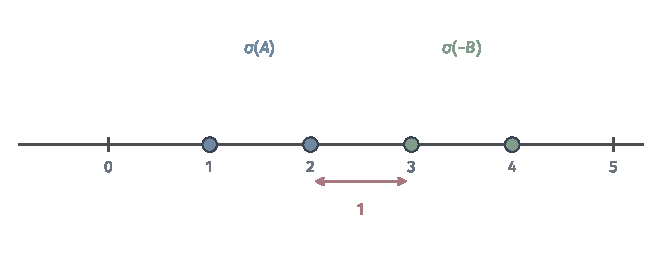
\includegraphics[width=112mm]{figures/00-shared/mathematical-preliminaries-upper/02-linear-spaces/matplotlib/ls-sylvester-separation/ls-sylvester-separation.pdf}
  \caption{谱分离条件的实轴示意。$\bm A=\operatorname{diag}(1,2)$的特征值$\{1,2\}$与$-\bm B$（$\bm B=\operatorname{diag}(-3,-4)$）的特征值$\{3,4\}$不相交，最近一对相距$1$，所以四个分母$\lambda_i+\mu_j$都不为零，对任意$\bm C$方程都有唯一解。}
  \label{fig:ls-sylvester-separation}
\end{figure}

\begin{theorem}[Sylvester方程的唯一可解性]
\label{thm:ls-sylvester-unique-solvability}
设$\bm A\in\mathbb R^{m\times m}$、$\bm B\in\mathbb R^{d\times d}$。方程$\bm A\bm X+\bm X\bm B=\bm C$对每个$\bm C\in\mathbb R^{m\times d}$都有唯一解，当且仅当
\begin{equation}
 \operatorname{spec}(\bm A)\cap\operatorname{spec}(-\bm B)=\varnothing ,
 \label{eq:ls-sylvester-spectral-separation}
\end{equation}
即对$\bm A$的任一特征值$\lambda$与$\bm B$的任一特征值$\mu$，都有$\lambda+\mu\neq0$。
\end{theorem}

\begin{proof}
$\mathcal L$把$\mathbb R^{m\times d}$映到自身。由秩零度定理，它对每个右端唯一可解，当且仅当齐次方程只有零解，也就是$\det\bm K\neq0$。这个行列式在实数域和复数域中是同一个数，所以可以在复数域中讨论齐次方程。

必要性。设$\bm A\bm u=\lambda\bm u$，且$-\lambda$是$\bm B$的特征值。$\bm B^\top$与$\bm B$有相同的特征多项式，所以$-\lambda$也是$\bm B^\top$的特征值，可取$\bm B^\top\bm w=-\lambda\bm w$，其中$\bm u,\bm w\neq\bm0$。于是$\bm X=\bm u\bm w^\top\neq\bm0$满足$\bm A\bm X+\bm X\bm B=\lambda\bm u\bm w^\top+\bm u(\bm B^\top\bm w)^\top=\lambda\bm u\bm w^\top-\lambda\bm u\bm w^\top=\bm0$，齐次方程有非零解。

充分性。设$\bm A\bm X+\bm X\bm B=\bm0$，即$\bm A\bm X=\bm X(-\bm B)$。归纳得$\bm A^k\bm X=\bm X(-\bm B)^k$，从而对任意多项式$p$有$p(\bm A)\bm X=\bm X\,p(-\bm B)$。取$p(z)=\prod_k(z-\lambda_k)$为$\bm A$的特征多项式，由Cayley--Hamilton定理~\ref{thm:ls-cayley-hamilton}，$p(\bm A)=\bm0$。另一方面，$p(-\bm B)=\prod_k(-\bm B-\lambda_k\bm I)$中每个$\lambda_k$都不是$-\bm B$的特征值，各因子可逆，所以$p(-\bm B)$可逆。于是$\bm X\,p(-\bm B)=\bm0$推出$\bm X=\bm0$。
\end{proof}

这一条件与$\bm A$、$\bm B$各自是否可逆无关。$\bm A=\bm0$、$\bm B=\bm I_d$时$\bm A$不可逆，方程却化为$\bm X=\bm C$，唯一可解；$1\times1$情形$\bm A=2$、$\bm B=-2$都可逆，方程却是$0\cdot x=c$。

谱不相交只回答解是否唯一，不回答解对数据误差是否敏感。对角情形下，最小的$|\lambda_i+\mu_j|$越接近零，$\bm C$的误差被放大得越多；矩阵远离正规时，即使所有谱和都远离零，解仍可能很敏感，第~\ref{sec:ls-sylvester-diagonalizable}节会看到其中的原因。

\subsection{Schur分解法}
\label{sec:ls-sylvester-schur}

稠密的一般Sylvester方程通常用\term{Bartels--Stewart算法}（Bartels--Stewart algorithm）求解。它的思路与解三角方程组相同：先用正交相似把两个系数化为准上三角形，未知元之间就有了先后依赖，可以逐个回代。下面设谱条件~\eqref{eq:ls-sylvester-spectral-separation}成立，依次说明变换、回代次序和二阶块的处理，再给出算法步骤、算例与分析。

\paragraph{主要思想：正交变换到准三角形}
第一步，分别对两个系数作实Schur分解（定理~\ref{thm:ls-real-schur}）
\[
 \bm A=\bm U\bm T\bm U^\top,\qquad \bm B=\bm V\bm S\bm V^\top,
\]
其中$\bm U,\bm V$正交，$\bm T,\bm S$是准上三角矩阵，对角块为$1\times1$（实特征值）或$2\times2$（一对共轭复特征值）。这一步只依赖$\bm A$、$\bm B$，与右端无关。

把分解代入$\bm A\bm X+\bm X\bm B=\bm C$，得$\bm U\bm T\bm U^\top\bm X+\bm X\bm V\bm S\bm V^\top=\bm C$。两边左乘$\bm U^\top$、右乘$\bm V$，利用$\bm U^\top\bm U=\bm I$、$\bm V^\top\bm V=\bm I$，并记$\bm Y=\bm U^\top\bm X\bm V$、$\bm D=\bm U^\top\bm C\bm V$，方程化为
\begin{equation}
 \bm T\bm Y+\bm Y\bm S=\bm D .
 \label{eq:ls-sylvester-transformed}
\end{equation}
$\bm T$与$\bm A$、$\bm S$与$\bm B$分别相似，特征值相同，所以新方程同样满足谱条件。正交变换还不改变Frobenius范数：任一近似解$\bm Z$在原坐标中的残差，等于$\bm W=\bm U^\top\bm Z\bm V$在新坐标中的残差（下面定理~\ref{thm:ls-bartels-stewart}的第三条）。因此在新坐标中解得准确，换回原坐标后残差不会被放大。

\paragraph{主要思想：上三角情形的回代次序}
先看$\bm T$、$\bm S$都是上三角的情形。比较式~\eqref{eq:ls-sylvester-transformed}两边的$(i,j)$元：$(\bm T\bm Y)_{i,j}=\sum_{k\geq i}t_{i,k}y_{k,j}$，$(\bm Y\bm S)_{i,j}=\sum_{\ell\leq j}y_{i,\ell}s_{\ell,j}$。把含$y_{i,j}$的两项留在左边，得
\begin{equation}
 (t_{i,i}+s_{j,j})\,y_{i,j}
 =d_{i,j}-\sum_{k>i}t_{i,k}y_{k,j}-\sum_{\ell<j}y_{i,\ell}s_{\ell,j}.
 \label{eq:ls-sylvester-triangular-entry}
\end{equation}
右端第一个和只用同一列中更靠下的元素，第二个和只用同一行中更靠左的元素。所以按列$j=1,\ldots,d$从左向右，每列内按行$i=m,\ldots,1$从下向上计算，每一步右端都已知。除数$t_{i,i}+s_{j,j}$是$\bm A$与$\bm B$的一对特征值之和，由谱条件不为零。

同一次序也可以按整列写出。$\bm Y\bm S$的第$j$列是$\sum_{\ell\leq j}s_{\ell,j}\bm y_\ell$，比较式~\eqref{eq:ls-sylvester-transformed}两边的第$j$列，得
\[
 (\bm T+s_{j,j}\bm I_m)\bm y_j=\bm d_j-\sum_{\ell<j}s_{\ell,j}\bm y_\ell .
\]
右端只用到更靠左的列；每列的系数是上三角矩阵，用第~\ref{sec:ls-lu}节的回代从最后一行向上求解，逐行展开正是式~\eqref{eq:ls-sylvester-triangular-entry}。图~\ref{fig:ls-bartels-stewart-column-order}画出了第$j$列的依赖：$\bm S$第$j$列中对角线以上的元素把已求出的列带进右端，对角元$s_{j,j}$并入当前列的三角系数。

\begin{figure}[htbp]
  \centering
  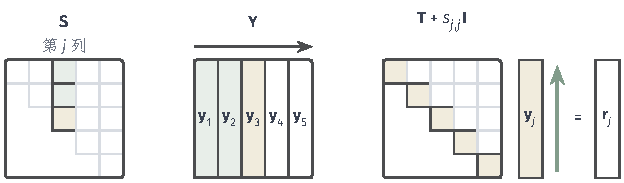
\includegraphics[width=109.6mm]{figures/01-basic-mathematics/03-vectors-matrices-and-multivariate-functions/tikz/c5-bartels-stewart-column-order/figure.pdf}
  \caption{Bartels--Stewart算法逐列求解$\bm T\bm Y+\bm Y\bm S=\bm D$的次序（上三角情形，图中取当前列$j=3$）。左：$\bm S$的第$j$列，绿色元素$s_{\ell,j}$（$\ell<j$）对应已求出的列，黄色为$s_{j,j}$。中：$\bm Y$的列从左到右求出。右：当前列解一个对角元为$t_{i,i}+s_{j,j}$的上三角方程组，从最后一行向上回代。}
  \label{fig:ls-bartels-stewart-column-order}
\end{figure}

\paragraph{主要思想：二阶对角块的局部系统}
实Schur形含$2\times2$对角块时，把一个标量未知数换成一个未知子块。按$\bm T$、$\bm S$的对角块把$\bm Y$、$\bm D$分块，记$\bm T$的第$I$个对角块为$\bm T_{I,I}$、$\bm S$的第$J$个对角块为$\bm S_{J,J}$，比较第$(I,J)$块得
\[
 \begin{aligned}
 \bm T_{I,I}\bm Y_{I,J}+\bm Y_{I,J}\bm S_{J,J}
 &=\bm D_{I,J}-\sum_{K>I}\bm T_{I,K}\bm Y_{K,J}\\
 &\quad-\sum_{L<J}\bm Y_{I,L}\bm S_{L,J}.
 \end{aligned}
\]
右端只含同一块列中更靠下的块和更靠左的块列，因此按块列从左到右、每块列从下到上计算。

左边是一个小Sylvester方程，$\bm Y_{I,J}$至多是$2\times2$的，至多含四个未知数。由式~\eqref{eq:ls-sylvester-vectorized}，它的向量化系数是$\bm I\otimes\bm T_{I,I}+\bm S_{J,J}^\top\otimes\bm I$，至多为$4$阶，直接消元即可；只在这样的局部形成Kronecker系数。$\bm T_{I,I}$的特征值是$\bm A$的特征值，$\bm S_{J,J}$的特征值是$\bm B$的特征值，所以局部方程满足谱条件，由定理~\ref{thm:ls-sylvester-unique-solvability}唯一可解。

\paragraph{算法实现}
把上面三步连起来，Bartels--Stewart算法如下。
\begin{enumerate}
 \item 计算实Schur分解$\bm A=\bm U\bm T\bm U^\top$、$\bm B=\bm V\bm S\bm V^\top$，并变换右端$\bm D=\bm U^\top\bm C\bm V$。
 \item 按块列从左到右、每块列从下到上的次序，对每个块$(I,J)$从$\bm D_{I,J}$中减去已求出块的贡献，再解至多四个未知数的局部方程，得$\bm Y_{I,J}$。
 \item 恢复原未知量$\bm X=\bm U\bm Y\bm V^\top$，并在原方程中计算残差$\bm A\bm X+\bm X\bm B-\bm C$。精确算术下它为零；浮点计算中它的Frobenius范数与新坐标中的残差相同，可以直接用来检验整个流程。
\end{enumerate}
局部方程的系数接近奇异时，除法会放大误差，中间量也可能溢出。数值软件库中的实现因此常引入一个缩放因子$\sigma\in(0,1]$，实际求解$\bm T\bm Y+\bm Y\bm S=\sigma\bm D$，再连同$\sigma$一起返回，并对过小的局部分母给出警告。使用者应把$\sigma<1$或这类警告视为方程接近不可解的信号，而不是忽略它。

\begin{example}[Schur形方程的逐元素回代]
\label{ex:ls-sylvester-schur-form-entries}
先跳过Schur分解，直接从已为Schur形的系数出发，看逐元素回代应按什么次序进行。取
\[
 \bm T=\begin{bmatrix}1&2\\0&3\end{bmatrix},\quad
 \bm S=\begin{bmatrix}4&1\\0&5\end{bmatrix},\quad
 \bm D=\begin{bmatrix}11&21\\21&35\end{bmatrix}.
\]
谱和$t_{i,i}+s_{j,j}$为$5,6,7,8$，都不为零，每个局部方程都可以相除。按式~\eqref{eq:ls-sylvester-triangular-entry}，第$1$列从下向上：
\[
 y_{2,1}=\frac{21}{3+4}=3,\qquad
 y_{1,1}=\frac{11-t_{1,2}y_{2,1}}{1+4}=\frac{11-2\cdot3}{5}=1 .
\]
第$2$列从下向上，右端还要减去左边一列经$s_{1,2}=1$带来的贡献：
\[
 \begin{aligned}
 y_{2,2}&=\frac{35-y_{2,1}s_{1,2}}{3+5}=\frac{35-3}{8}=4,\\
 y_{1,2}&=\frac{21-t_{1,2}y_{2,2}-y_{1,1}s_{1,2}}{1+5}=\frac{21-8-1}{6}=2 .
 \end{aligned}
\]
于是$\bm Y=\bigl[\begin{smallmatrix}1&2\\3&4\end{smallmatrix}\bigr]$。代回全部四个元素：$\bm T\bm Y=\bigl[\begin{smallmatrix}7&10\\9&12\end{smallmatrix}\bigr]$，$\bm Y\bm S=\bigl[\begin{smallmatrix}4&11\\12&23\end{smallmatrix}\bigr]$，和为$\bigl[\begin{smallmatrix}11&21\\21&35\end{smallmatrix}\bigr]=\bm D$。若次序颠倒，例如先算$y_{1,1}$，它的右端需要尚未求出的$y_{2,1}$，回代无法进行。
\end{example}

上例跳过了Schur分解。下面的例子从一般系数出发，完整走一遍变换、回代和恢复。

\begin{example}[Bartels--Stewart求解一个二阶方程]
\label{ex:ls-bartels-stewart-2x2}
取
\[
 \bm A=\begin{bmatrix}-2&3\\-4&5\end{bmatrix},\quad
 \bm B=\begin{bmatrix}1&1\\0&3\end{bmatrix},\quad
 \bm C=\begin{bmatrix}1&12\\-2&21\end{bmatrix}.
\]
$\bm A$的特征值为$2,1$，$-\bm B$的特征值为$-1,-3$，谱条件成立。实Schur分解：由$\bm A(3,4)^\top=2(3,4)^\top$取$\bm U=\tfrac15\bigl[\begin{smallmatrix}3&-4\\4&3\end{smallmatrix}\bigr]$，得$\bm T=\bm U^\top\bm A\bm U=\bigl[\begin{smallmatrix}2&7\\0&1\end{smallmatrix}\bigr]$；$\bm B$已是上三角，取$\bm V=\bm I$、$\bm S=\bm B$。变换右端得$\bm D=\bm U^\top\bm C=\bigl[\begin{smallmatrix}-1&24\\-2&3\end{smallmatrix}\bigr]$。

在Schur坐标下逐列求解。第$1$列解$(\bm T+s_{1,1}\bm I)\bm y_1=\bm d_1$，即$\bigl[\begin{smallmatrix}3&7\\0&2\end{smallmatrix}\bigr]\bm y_1=(-1,-2)^\top$，从下往上得$y_{2,1}=-1$、$y_{1,1}=2$；第$2$列的右端为$\bm d_2-s_{1,2}\bm y_1=(24,3)^\top-(2,-1)^\top=(22,4)^\top$，解$\bigl[\begin{smallmatrix}5&7\\0&4\end{smallmatrix}\bigr]\bm y_2=(22,4)^\top$得$y_{2,2}=1$、$y_{1,2}=3$。变回原坐标，
\[
 \bm X=\bm U\bm Y=\frac15\begin{bmatrix}3&-4\\4&3\end{bmatrix}\begin{bmatrix}2&3\\-1&1\end{bmatrix}=\begin{bmatrix}2&1\\1&3\end{bmatrix}.
\]
核验：$\bm A\bm X=\bigl[\begin{smallmatrix}-1&7\\-3&11\end{smallmatrix}\bigr]$，$\bm X\bm B=\bigl[\begin{smallmatrix}2&5\\1&10\end{smallmatrix}\bigr]$，和为$\bm C$，原方程残差为零。
\end{example}

\paragraph{算法分析：正确性}
上面的推导说明每一步都能进行，而且按次序算出的块满足各自的块等式。把这些事实合在一起，就得到算法的正确性和残差检验的依据。

\begin{theorem}[Bartels--Stewart算法的正确性]
\label{thm:ls-bartels-stewart}
设$\bm A=\bm U\bm T\bm U^\top$、$\bm B=\bm V\bm S\bm V^\top$是实Schur分解，谱条件~\eqref{eq:ls-sylvester-spectral-separation}成立，$\bm D=\bm U^\top\bm C\bm V$。则
\begin{enumerate}
 \item 按块列从左到右、每块列从下到上的次序，每一步的局部方程$\bm T_{I,I}\bm Y_{I,J}+\bm Y_{I,J}\bm S_{J,J}=\bm E_{I,J}$都唯一可解，其中右端$\bm E_{I,J}$由已求出的块给出；
 \item 由此算出的$\bm Y$是方程~\eqref{eq:ls-sylvester-transformed}的唯一解，$\bm X=\bm U\bm Y\bm V^\top$是$\bm A\bm X+\bm X\bm B=\bm C$的唯一解；
 \item 对任意$\bm Z\in\mathbb R^{m\times d}$，记$\bm W=\bm U^\top\bm Z\bm V$，有$\lVert\bm A\bm Z+\bm Z\bm B-\bm C\rVert_{\mathrm F}=\lVert\bm T\bm W+\bm W\bm S-\bm D\rVert_{\mathrm F}$。
\end{enumerate}
\end{theorem}

\begin{proof}
先证第三条。由$\bm A=\bm U\bm T\bm U^\top$、$\bm B=\bm V\bm S\bm V^\top$与$\bm Z=\bm U\bm W\bm V^\top$，
\[
 \bm A\bm Z+\bm Z\bm B-\bm C=\bm U(\bm T\bm W+\bm W\bm S-\bm D)\bm V^\top,
\]
而左右乘正交矩阵不改变Frobenius范数。

再证第一条。准上三角矩阵的特征值是各对角块特征值的并，$\bm T$与$\bm A$相似，所以$\bm T_{I,I}$的特征值都是$\bm A$的特征值；同理$\bm S_{J,J}$的特征值都是$\bm B$的特征值。于是每个局部方程满足谱条件，由定理~\ref{thm:ls-sylvester-unique-solvability}唯一可解。

最后证第二条。第$(I,J)$块等式的右端只含按次序已算出的块，所以算出的每一块都满足相应的块等式；全部块等式合起来就是式~\eqref{eq:ls-sylvester-transformed}。$\bm T$、$\bm S$满足谱条件，由定理~\ref{thm:ls-sylvester-unique-solvability}，这个解唯一。在第三条中取$\bm Z=\bm X$、$\bm W=\bm Y$，得原方程残差为零；原方程的唯一性同样由该定理给出。
\end{proof}

\paragraph{算法分析：计算代价}
实Schur分解靠迭代算出，常用实现计入正交因子约需$25m^3$与$25d^3$次运算\scite{math-golub2013matrix}。变换右端与变回原坐标各约$2(m^2d+md^2)$次，逐块回代约$m^2d+md^2$次；存储只需$O(m^2+d^2+md)$个数。$m=d=100$时总量约$6\times10^7$次，而对式~\eqref{eq:ls-sylvester-vectorized}作稠密LU约需$7\times10^{11}$次，并要存储$10^8$个数。多组右端共用$\bm A$、$\bm B$时，两个Schur分解只做一次，每增加一个右端只增加$O(m^2d+md^2)$次运算。

\subsection{特征基下的求解}
\label{sec:ls-sylvester-diagonalizable}

当$\bm A$、$\bm B$都可对角化时，可以换到各自的特征基，把方程化为式~\eqref{eq:ls-sylvester-diagonal-closed-form}的对角情形。设$\bm A=\bm P\bm\Lambda\bm P^{-1}$、$\bm B=\bm R\bm M\bm R^{-1}$，其中$\bm\Lambda=\operatorname{diag}(\lambda_i)$、$\bm M=\operatorname{diag}(\mu_j)$。这条路线公式最简短，代价是换基矩阵一般不正交。

\paragraph{主要思想：换到特征基}
记$\bm Y=\bm P^{-1}\bm X\bm R$、$\bm D=\bm P^{-1}\bm C\bm R$。方程左乘$\bm P^{-1}$、右乘$\bm R$，由$\bm P^{-1}\bm A=\bm\Lambda\bm P^{-1}$与$\bm B\bm R=\bm R\bm M$化为$\bm\Lambda\bm Y+\bm Y\bm M=\bm D$。这时各坐标完全解耦，逐元素得到
\[
 (\lambda_i+\mu_j)\,y_{i,j}=d_{i,j}.
\]
谱条件成立时所有分母非零，$y_{i,j}=d_{i,j}/(\lambda_i+\mu_j)$。若某个$\lambda_i+\mu_j=0$，就要区分两种情形：$d_{i,j}\neq0$时这个坐标无解，$d_{i,j}=0$时$y_{i,j}$是自由变量。注意检查的是变换后的$d_{i,j}$，而不是原右端的$c_{i,j}$。

\paragraph{主要思想：恢复原未知量}
恢复公式为$\bm X=\bm P\bm Y\bm R^{-1}$，次序与换基相反。与Schur路线不同，这里的换基矩阵$\bm P$、$\bm R$一般不正交：变换右端和还原解时，误差可能被放大$\kappa_2(\bm P)\kappa_2(\bm R)$量级，所以实现前要检查两组特征基的条件数（见下面的算法分析）。实矩阵有复特征值时，$\bm P$、$\bm R$为复矩阵，全程用复数运算，最后舍去舍入产生的虚部。

\paragraph{算法实现}
算法依次执行以下步骤。
\begin{enumerate}
 \item 核验两组特征基可逆且条件数可以接受；若特征基不满秩或接近奇异，改用第~\ref{sec:ls-sylvester-schur}节的Schur路线，不尝试直接求逆。
 \item 变换右端时不求逆：先对$\bm P$作LU分解，对$\bm C$的各列求解$\bm P\bm Z=\bm C$，再令$\bm D=\bm Z\bm R$。
 \item 逐项检查谱和$\lambda_i+\mu_j$并相除，得$\bm Y$。
 \item 先算$\bm W=\bm P\bm Y$，再利用$\bm R$的LU分解求解$\bm X\bm R=\bm W$，得$\bm X=\bm P\bm Y\bm R^{-1}$；最后在原方程中计算残差。
\end{enumerate}

\begin{example}[对角系数下的逐元素相除与零谱和]
\label{ex:ls-sylvester-diagonal-zero-sum}
取$\bm A=\operatorname{diag}(1,2)$、$\bm B=\operatorname{diag}(3,4)$、$\bm C=\bigl[\begin{smallmatrix}4&10\\15&24\end{smallmatrix}\bigr]$。这时$\bm P=\bm R=\bm I$，$\bm D=\bm C$，四个谱和为$1+3=4$、$1+4=5$、$2+3=5$、$2+4=6$。逐元素相除得
\[
 x_{1,1}=\frac44=1,\quad x_{1,2}=\frac{10}5=2,\quad
 x_{2,1}=\frac{15}5=3,\quad x_{2,2}=\frac{24}6=4,
\]
即$\bm X=\bigl[\begin{smallmatrix}1&2\\3&4\end{smallmatrix}\bigr]$。四个元素互不耦合，每个只需一次除法。代回：$\bm A\bm X=\bigl[\begin{smallmatrix}1&2\\6&8\end{smallmatrix}\bigr]$，$\bm X\bm B=\bigl[\begin{smallmatrix}3&8\\9&16\end{smallmatrix}\bigr]$，和为$\bm C$。

再把右下角的谱和改为零：令$\bm B=\operatorname{diag}(3,-2)$，则$\lambda_2+\mu_2=0$，其余三个谱和$4,-1,5$仍非零。第$(2,2)$个方程变为$0\cdot x_{2,2}=c_{2,2}$。右端保持$c_{2,2}=24\neq0$时，方程无解；把右端改为$c_{2,2}=0$时，$x_{1,1},x_{1,2},x_{2,1}$仍由各自的除法唯一确定，$x_{2,2}$可以任取，解集是一条直线。
\end{example}

对角系数无须换基。下面的例子换到非正交的特征基，再除以谱和、还原。

\begin{example}[特征基下的逐元素求解]
\label{ex:ls-sylvester-eigenbasis}
取
\[
 \bm A=\begin{bmatrix}1&1\\0&2\end{bmatrix},\quad
 \bm B=\begin{bmatrix}3&1\\0&4\end{bmatrix},\quad
 \bm C=\begin{bmatrix}7&12\\15&21\end{bmatrix}.
\]
两者的特征向量都是$(1,0)^\top$与$(1,1)^\top$，故$\bm P=\bm R=\bigl[\begin{smallmatrix}1&1\\0&1\end{smallmatrix}\bigr]$，特征值分别为$1,2$与$3,4$，四个分母$\lambda_i+\mu_j$为$4,5,5,6$。换基、逐元素相除、再变回，依次得
\[
 \begin{gathered}
 \bm D=\bm P^{-1}\bm C\bm R=\begin{bmatrix}-8&-17\\15&36\end{bmatrix},\qquad
 \bm Y=\begin{bmatrix}-2&-17/5\\3&6\end{bmatrix},\\
 \bm X=\bm P\bm Y\bm R^{-1}=\begin{bmatrix}1&8/5\\3&3\end{bmatrix}.
 \end{gathered}
\]
代回有$\bm A\bm X=\bigl[\begin{smallmatrix}4&23/5\\6&6\end{smallmatrix}\bigr]$、$\bm X\bm B=\bigl[\begin{smallmatrix}3&37/5\\9&15\end{smallmatrix}\bigr]$，和为$\bm C$，残差为零。

若把$\bm B$的$(1,1)$元改为$-2$，则$\mu_1=-2$，$\lambda_2+\mu_1=0$。这时$\bm B$的特征基也随之改变，第$(2,1)$个方程变为$0\cdot y_{2,1}=d_{2,1}$，其中$d_{2,1}$是按新的特征基变换后的右端：$d_{2,1}\neq0$时无解，$d_{2,1}=0$时解不唯一。
\end{example}

\paragraph{算法分析：数值敏感度}
这条路线只在特征基接近正交时可靠。记$\delta_{\min}=\min_{i,j}|\lambda_i+\mu_j|$，则$\lVert\bm Y\rVert_{\mathrm F}\leq\lVert\bm D\rVert_{\mathrm F}/\delta_{\min}$。再对$\bm D=\bm P^{-1}\bm C\bm R$与$\bm X=\bm P\bm Y\bm R^{-1}$使用$\lVert\bm M_1\bm Z\bm M_2\rVert_{\mathrm F}\leq\lVert\bm M_1\rVert_2\lVert\bm Z\rVert_{\mathrm F}\lVert\bm M_2\rVert_2$，只能得到
\[
 \lVert\bm X\rVert_{\mathrm F}
 \leq\frac{\kappa_2(\bm P)\,\kappa_2(\bm R)}{\delta_{\min}}\lVert\bm C\rVert_{\mathrm F},
\]
所以在斜基下，谱和远离零并不独自保证良好条件。

换基本身也会放大误差：$\bm P^{-1}\bm C$的元素可以比$\bm C$大$\kappa_2(\bm P)$量级，变回时再相互抵消。例如$0<\epsilon\ll1$时，$\bm A=\bigl[\begin{smallmatrix}1&1\\0&1+\epsilon\end{smallmatrix}\bigr]$的特征向量$(1,0)^\top$与$(1,\epsilon)^\top$几乎平行，$\kappa_2(\bm P)\geq1/\epsilon$，中间量的大小约为$1/\epsilon$，舍入误差随之被放大。

$\bm A$、$\bm B$实对称时，谱定理~\ref{thm:ls-real-symmetric-spectral}给出正交特征基，$\kappa_2=1$，元素公式既简单又可靠。一般情形即使可以对角化，也宜使用第~\ref{sec:ls-sylvester-schur}节的正交Schur变换。

% 矩阵方程（二）：Lyapunov方程X-A^TXA=Q与A^TX+XA=-Q（离散累计与唯一可解条件、一次Schur变换下的对称递推与检验、级数解、半正定右端的正定条件与谱证书）

\section{Lyapunov方程}
\label{sec:ls-lyapunov}

第~\ref{chap:linear-recurrence-stability}章研究了反复作用$\bm x_{k+1}=\bm A\bm x_k$的长期行为。若每一步以二次量$\bm x_k^\top\bm Q\bm x_k$计量状态的大小，能否用一个矩阵$\bm X$直接写出全部步骤的累计量$\bm x_0^\top\bm X\bm x_0$？本节由这一离散累计引出Lyapunov方程，并把相应的连续型方程作为Sylvester方程的特例处理。

全节统一采用两种写法：离散型$\bm X-\bm A^\top\bm X\bm A=\bm Q$，连续型$\bm A^\top\bm X+\bm X\bm A=-\bm Q$，其中$\bm Q$对称，未知量$\bm X$与上一节一样记为$\bm X$。两者都是左乘$\bm A^\top$、右乘$\bm A$，所以只需对$\bm A$作一次Schur分解，回代次序也相同。离散型的正定性论证只用矩阵幂和级数；连续型正定解的积分证明需要矩阵指数，本节只陈述条件并给出代数检验。

\subsection{离散型与连续型方程}
\label{sec:ls-lyapunov-solvability}

设$\bm A\in\mathbb R^{d\times d}$，$\bm Q=\bm Q^\top\succeq0$，$\bm x_k=\bm A^k\bm x_0$。前$N+1$步的累计量为
\[
 \sum_{k=0}^{N}\bm x_k^\top\bm Q\bm x_k=\bm x_0^\top\bm X_N\bm x_0,\qquad
 \bm X_N=\sum_{k=0}^{N}(\bm A^\top)^k\bm Q\bm A^k ,
\]
其中$\bm X_N$与初值无关。把和式的首项单独写出，其余各项提出左右的$\bm A^\top$与$\bm A$，得递推$\bm X_{N+1}=\bm Q+\bm A^\top\bm X_N\bm A$。若$\bm X_N$收敛到$\bm X$，对递推取极限，极限应满足离散型\term{Lyapunov方程}（Lyapunov equation）
\begin{equation}
 \bm X-\bm A^\top\bm X\bm A=\bm Q .
 \label{eq:ls-discrete-lyapunov}
\end{equation}
它是矩阵空间上固定更新$\bm X\mapsto\bm Q+\bm A^\top\bm X\bm A$的不动点方程。

方程~\eqref{eq:ls-discrete-lyapunov}也可以逐步读出。若$\bm X$是解，则沿轨迹有
\[
 \bm x_{k+1}^\top\bm X\bm x_{k+1}-\bm x_k^\top\bm X\bm x_k
 =\bm x_k^\top(\bm A^\top\bm X\bm A-\bm X)\bm x_k
 =-\bm x_k^\top\bm Q\bm x_k ,
\]
即二次量$\bm x^\top\bm X\bm x$每走一步恰好减少这一步的计量$\bm x_k^\top\bm Q\bm x_k$。把这些等式从$k=0$加到$N$，就回到上面的累计量。

离散型方程不是替换系数后的Sylvester方程：左边是恒等作用减去双侧作用，向量化后的系数矩阵为$\bm I-\bm A^\top\otimes\bm A^\top$。相应地，唯一可解的条件由特征值的乘积而不是和决定。下面的定理对两侧系数不同的一般形式陈述，后面处理Schur形的局部块时要用到这一形式。

\begin{theorem}[离散型方程的唯一可解性]
\label{thm:ls-discrete-lyapunov-unique}
设$\bm G\in\mathbb R^{m\times m}$、$\bm H\in\mathbb R^{d\times d}$。方程$\bm Y-\bm G^\top\bm Y\bm H=\bm E$对每个$\bm E\in\mathbb R^{m\times d}$都有唯一解，当且仅当对$\bm G$的任一特征值$\lambda$与$\bm H$的任一特征值$\mu$，都有$\lambda\mu\neq1$。特别地，方程~\eqref{eq:ls-discrete-lyapunov}对每个$\bm Q$唯一可解，当且仅当$\bm A$在复数域中的任意两个特征值$\lambda,\lambda'$（可以是同一个）满足$\lambda\lambda'\neq1$；此时若$\bm Q$对称，则解对称。
\end{theorem}

\begin{proof}
与定理~\ref{thm:ls-sylvester-unique-solvability}的证明一样，向量化后的系数矩阵是实矩阵，唯一可解等价于它的行列式非零，所以只需在复数域中判断齐次方程$\bm Y=\bm G^\top\bm Y\bm H$是否只有零解。

必要性。设$\lambda\mu=1$。$\bm G^\top$与$\bm G$、$\bm H^\top$与$\bm H$的特征值分别相同，可取非零向量$\bm w,\bm v$使$\bm G^\top\bm w=\lambda\bm w$、$\bm H^\top\bm v=\mu\bm v$。令$\bm Y=\bm w\bm v^\top\neq\bm0$，则$\bm Y\bm H=\bm w(\bm H^\top\bm v)^\top=\mu\bm Y$，于是$\bm G^\top\bm Y\bm H=\lambda\mu\bm Y=\bm Y$，齐次方程有非零解。

充分性要用复数域中的三角化。把定理~\ref{thm:ls-real-schur}证明中的归纳搬到复数域：复方阵总有复特征向量，每一步取它张成的一维不变子空间，用标准正交基扩充成酉矩阵（第~\ref{sec:ls-adjoints}节），就得到$\bm G=\bm W_1\bm R_1\bm W_1^*$、$\bm H=\bm W_2\bm R_2\bm W_2^*$，其中$\bm W_1,\bm W_2$为酉矩阵，$\bm R_1,\bm R_2$上三角，对角元分别是$\bm G$、$\bm H$的特征值。$\bm G$是实矩阵，$\bm G^\top=\bm G^*=\bm W_1\bm R_1^*\bm W_1^*$。

设$\bm Y=\bm G^\top\bm Y\bm H$，令$\bm Z=\bm W_1^*\bm Y\bm W_2$，则$\bm Z=\bm R_1^*\bm Z\bm R_2$。$\bm R_1^*$是下三角矩阵，其$(i,k)$元为$\overline{(\bm R_1)_{k,i}}$，所以比较$(i,j)$元得
\[
 \bigl(1-\overline{(\bm R_1)_{i,i}}\,(\bm R_2)_{j,j}\bigr)z_{i,j}
 =\sum_{\substack{k\leq i,\ \ell\leq j\\(k,\ell)\neq(i,j)}}\overline{(\bm R_1)_{k,i}}\,z_{k,\ell}\,(\bm R_2)_{\ell,j}.
\]
实矩阵的非实特征值成共轭对出现，所以$\overline{(\bm R_1)_{i,i}}$仍是$\bm G$的特征值，左边系数按假设非零。右端各项满足$k+\ell<i+j$。对$i+j$归纳：$i+j=2$时右端为空，$z_{1,1}=0$；若下标和较小的元素都为零，右端为零，于是$z_{i,j}=0$。所以$\bm Z=\bm0$，$\bm Y=\bm0$。

取$\bm G=\bm H=\bm A$即得关于方程~\eqref{eq:ls-discrete-lyapunov}的结论。若$\bm Q$对称，对方程转置，由$(\bm A^\top\bm X\bm A)^\top=\bm A^\top\bm X^\top\bm A$知$\bm X^\top$也是解，由唯一性$\bm X^\top=\bm X$。
\end{proof}

下面最常用的是$\rho(\bm A)<1$的情形。此时任意两个特征值满足$|\lambda\lambda'|<1$，条件自然成立；唯一性还可以不经三角化，直接由矩阵幂的衰减证明。后面的级数论证用的就是这一直接证明。

\begin{lemma}[谱半径小于一时的唯一性]
\label{lem:ls-discrete-lyapunov-uniqueness}
若谱半径$\rho(\bm A)<1$，则方程~\eqref{eq:ls-discrete-lyapunov}至多有一个解；若$\bm Q$对称且解存在，则解对称。
\end{lemma}

\begin{proof}
两个解之差$\bm X$满足$\bm X=\bm A^\top\bm X\bm A$。反复代入得$\bm X=(\bm A^\top)^k\bm X\bm A^k$，于是$\lVert\bm X\rVert_2\leq\lVert\bm A^k\rVert_2^2\lVert\bm X\rVert_2$；由定理~\ref{thm:ls-power-decay}，$\bm A^k\to\bm0$，故$\bm X=\bm0$。若$\bm Q$对称，对方程转置可知$\bm X^\top$也是解，由唯一性$\bm X^\top=\bm X$。
\end{proof}

级数$\sum_k(\bm A^\top)^k\bm Q\bm A^k$的收敛与正定性在第~\ref{sec:ls-lyapunov-positivity}节建立。

连续型方程对应状态随时间连续变化的情形。若状态按$\dot{\bm x}=\bm A\bm x$演化（这类方程的解理论在后续卷中建立），由乘积的求导法则，二次量$\bm x^\top\bm X\bm x$的变化率为$\bm x^\top(\bm A^\top\bm X+\bm X\bm A)\bm x$。要求它恰好等于$-\bm x^\top\bm Q\bm x$，就得到连续型Lyapunov方程
\begin{equation}
 \bm A^\top\bm X+\bm X\bm A=-\bm Q .
 \label{eq:ls-continuous-lyapunov}
\end{equation}
这一段只用来说明方程的来历，本章不使用连续演化的任何结论。在代数上，它是Sylvester方程取左系数$\bm A^\top$、右系数$\bm A$、右端$-\bm Q$的特例。$\bm A^\top$与$\bm A$的特征值相同，所以Sylvester方程的谱条件在这里变成$\bm A$自身特征值两两之和的条件。

\begin{theorem}[连续型Lyapunov方程的唯一可解性]
\label{thm:ls-continuous-lyapunov-unique}
设$\bm A\in\mathbb R^{d\times d}$。方程~\eqref{eq:ls-continuous-lyapunov}对每个$\bm Q\in\mathbb R^{d\times d}$都有唯一解，当且仅当对$\bm A$在复数域中的任意两个特征值$\lambda,\lambda'$（可以是同一个），都有$\lambda+\lambda'\neq0$。此时若$\bm Q$对称，则解$\bm X$也对称。
\end{theorem}

\begin{proof}
在定理~\ref{thm:ls-sylvester-unique-solvability}中取左系数$\bm A^\top$、右系数$\bm A$。$\operatorname{spec}(\bm A^\top)=\operatorname{spec}(\bm A)$，$\operatorname{spec}(-\bm A)=\{-\lambda:\lambda\in\operatorname{spec}(\bm A)\}$，所以条件~\eqref{eq:ls-sylvester-spectral-separation}恰好是任意两个特征值之和不为零，由该定理得第一部分。若$\bm Q$对称，对方程转置得$\bm X^\top\bm A+\bm A^\top\bm X^\top=-\bm Q$，$\bm X^\top$也是解，由唯一性$\bm X^\top=\bm X$。
\end{proof}

$\bm A$的特征值实部全负时，任意两个之和的实部为负，唯一性成立。但这只是充分条件：例如$\bm A=\operatorname{diag}(1,2)$的谱和$2,3,4$都不为零，方程同样唯一可解。离散型的对应情形是：$\rho(\bm A)<1$是$\lambda\lambda'\neq1$的充分条件而非必要条件，$\bm A=\operatorname{diag}(2,3)$的各个乘积$4,6,9$都不等于$1$。两种条件的强化形式（实部全负、谱半径小于一）在第~\ref{sec:ls-lyapunov-positivity}节决定解是否正定。

\subsection{对称解的计算与检验}
\label{sec:ls-lyapunov-solve}

两类方程都可以看成Sylvester型方程，直接套用第~\ref{sec:ls-sylvester-schur}节的算法也能求解。但那样做要对$\bm A$与$\bm A^\top$分别分解，也没有利用解的对称性。本节只作一次Schur分解，并只求解的上三角部分。

\paragraph{主要思想：一次Schur变换}
对$\bm A$作实Schur分解$\bm A=\bm U\bm T\bm U^\top$，则$\bm A^\top=\bm U\bm T^\top\bm U^\top$。令$\bm Y=\bm U^\top\bm X\bm U$、$\bm D=\bm U^\top\bm Q\bm U$，$\bm D$仍对称。把分解代入方程~\eqref{eq:ls-continuous-lyapunov}与~\eqref{eq:ls-discrete-lyapunov}，左乘$\bm U^\top$、右乘$\bm U$，分别得
\[
 \bm T^\top\bm Y+\bm Y\bm T=-\bm D,\qquad
 \bm Y-\bm T^\top\bm Y\bm T=\bm D .
\]
$\bm X$对称当且仅当$\bm Y$对称，唯一可解时$\bm Y$确实对称，所以只需求$i\leq j$的元素$y_{i,j}$，下三角部分由$y_{j,i}=y_{i,j}$填入。下面先设$\bm T$上三角。

\paragraph{主要思想：连续型的逐元素递推}
$\bm T^\top$是下三角矩阵，$(\bm T^\top\bm Y)_{i,j}=\sum_{k\leq i}t_{k,i}y_{k,j}$；$(\bm Y\bm T)_{i,j}=\sum_{k\leq j}y_{i,k}t_{k,j}$。把含$y_{i,j}$的两项留在左边，得
\begin{equation}
 (t_{i,i}+t_{j,j})\,y_{i,j}
 =-d_{i,j}-\sum_{k<i}t_{k,i}y_{k,j}-\sum_{k<j}y_{i,k}t_{k,j}.
 \label{eq:ls-continuous-lyapunov-entry}
\end{equation}
按列$j=1,\ldots,d$从左向右，每列内按行$i=1,\ldots,j$从上到对角元计算。检查右端用到的元素：$y_{k,j}$（$k<i$）在同一列更靠上，已经求出；$y_{i,k}$（$k<j$）按对称性改写为上三角位置后，所在列号不超过$j$，列号等于$j$时只可能是$i=j$、行号$k<j$，也已求出。除数$t_{i,i}+t_{j,j}$是$\bm A$的两个特征值之和，由定理~\ref{thm:ls-continuous-lyapunov-unique}的条件不为零。

这一次序不能照搬第~\ref{sec:ls-sylvester-schur}节。那里左系数$\bm T$是上三角，依赖指向同列更靠下的元素，每列从下向上；这里左系数换成下三角的$\bm T^\top$，依赖指向同列更靠上的元素，所以每列从上向下。

\paragraph{主要思想：离散型的逐元素递推}
离散型中
\[
 (\bm T^\top\bm Y\bm T)_{i,j}=\sum_{k\leq i,\ \ell\leq j}t_{k,i}\,y_{k,\ell}\,t_{\ell,j},
\]
其中只有$(k,\ell)=(i,j)$一项含$y_{i,j}$。把它移到左边，得
\begin{equation}
 (1-t_{i,i}t_{j,j})\,y_{i,j}
 =d_{i,j}+\sum_{\substack{k\leq i,\ \ell\leq j\\(k,\ell)\neq(i,j)}}t_{k,i}\,y_{k,\ell}\,t_{\ell,j}.
 \label{eq:ls-discrete-lyapunov-entry}
\end{equation}
采用与连续型相同的次序。右端的$y_{k,\ell}$满足$k\leq i\leq j$、$\ell\leq j$；按对称性写成上三角位置后，所在列号$\max(k,\ell)\leq j$。列号小于$j$的元素在前面的列中已经求出；列号等于$j$时，要么$\ell=j$、$k<i$，要么$k=i=j$、$\ell<j$，两种情形都是当前列更靠上的元素。所以同一列序只读取已求元素。除数$1-t_{i,i}t_{j,j}$由定理~\ref{thm:ls-discrete-lyapunov-unique}的条件不为零。

\paragraph{主要思想：整列形式与对称性}
若不利用对称性、把整列$\bm y_j$作为未知量，两类方程按列分别写成
\[
 (\bm T^\top+t_{j,j}\bm I)\bm y_j=-\bm d_j-\sum_{\ell<j}t_{\ell,j}\bm y_\ell,\qquad
 (\bm I-t_{j,j}\bm T^\top)\bm y_j=\bm d_j+\bm T^\top\sum_{\ell<j}t_{\ell,j}\bm y_\ell .
\]
右端只用到更靠左的列，系数是下三角矩阵，每列从上到下前代。这样要求全部$d^2$个元素。若只求上三角部分，右端中左边各列的下三角元素$y_{i,\ell}$（$i>\ell$）就要取为$y_{\ell,i}$，其中$i=j$的元素恰好位于当前列，是正在求解的未知量。所以利用对称性时应按式~\eqref{eq:ls-continuous-lyapunov-entry}与~\eqref{eq:ls-discrete-lyapunov-entry}逐元素推进，未知量从$d^2$个减为$d(d+1)/2$个。

\paragraph{主要思想：二阶块与局部算子}
$\bm T$含$2\times2$对角块时，把相应的行和列成对处理。记$\bm T$的对角块为$\bm T_{I,I}$，按块写出的两类局部方程为
\[
 \begin{aligned}
 \bm T_{I,I}^\top\bm Y_{I,J}+\bm Y_{I,J}\bm T_{J,J}
 &=-\bm D_{I,J}-\sum_{K<I}\bm T_{K,I}^\top\bm Y_{K,J}-\sum_{K<J}\bm Y_{I,K}\bm T_{K,J},\\
 \bm Y_{I,J}-\bm T_{I,I}^\top\bm Y_{I,J}\bm T_{J,J}
 &=\bm D_{I,J}+\sum_{\substack{K\leq I,\ L\leq J\\(K,L)\neq(I,J)}}\bm T_{K,I}^\top\bm Y_{K,L}\bm T_{L,J}.
 \end{aligned}
\]
每个局部方程至多含四个未知数，向量化后直接消元。对角块$I=J$时$\bm Y_{I,I}$对称，只需存三个未知量。局部算子的可逆性分别由定理~\ref{thm:ls-sylvester-unique-solvability}（左系数$\bm T_{I,I}^\top$、右系数$\bm T_{J,J}$）与定理~\ref{thm:ls-discrete-lyapunov-unique}（$\bm G=\bm T_{I,I}$、$\bm H=\bm T_{J,J}$）给出：两块的特征值都是$\bm A$的特征值，所以标量情形的“分母非零”推广为“局部算子可逆”。与Sylvester方程一样，局部系数接近奇异时实现中应保留缩放因子并给出条件警告。

\paragraph{算法实现}
算法依次执行以下步骤。
\begin{enumerate}
 \item 检查$\bm Q$是否对称；不对称的输入不属于本节的问题。
 \item 计算$\bm A=\bm U\bm T\bm U^\top$与$\bm D=\bm U^\top\bm Q\bm U$。
 \item 按块列从左到右、每块列从上到对角块的次序，累计已知项，解局部方程，并把$\bm Y_{I,J}^\top$镜像填入$\bm Y_{J,I}$。
 \item 恢复$\bm X=\bm U\bm Y\bm U^\top$，在原坐标中检查残差、对称性，以及问题要求的正定性。
\end{enumerate}
第四步必须在原方程中进行，只检查变换后的小系统是不够的。也不能把算出的非对称误差强行平均后就宣布成功，对称化与残差检验回答的是不同的问题（见本节末的检验）。

\begin{example}[连续型方程的逐元素递推]
\label{ex:ls-continuous-lyapunov-entries}
取$\bm A=\bigl[\begin{smallmatrix}-1&1\\0&-2\end{smallmatrix}\bigr]$、$\bm Q=\bm I$。$\bm A$已是上三角，取$\bm U=\bm I$、$\bm T=\bm A$、$\bm D=\bm I$；特征值$-1,-2$两两之和$-2,-3,-4$都不为零。记$\bm X=\bigl[\begin{smallmatrix}p&q\\q&r\end{smallmatrix}\bigr]$，按式~\eqref{eq:ls-continuous-lyapunov-entry}依次计算：
\[
 \begin{aligned}
 (1,1):&\quad -2p=-1, & p&=\tfrac12,\\
 (1,2):&\quad -3q=-p\,t_{1,2}=-p, & q&=\tfrac16,\\
 (2,2):&\quad -4r=-1-t_{1,2}q-q\,t_{1,2}=-1-2q, & r&=\tfrac13 .
 \end{aligned}
\]
第二步就是$p-3q=0$，第三步就是$2q-4r=-1$。代回原方程：$\bm A^\top\bm X+\bm X\bm A=\bigl[\begin{smallmatrix}-2p&p-3q\\p-3q&2q-4r\end{smallmatrix}\bigr]=-\bm I$。解对称，且$p=\tfrac12>0$、$\det\bm X=\tfrac16-\tfrac1{36}=\tfrac5{36}>0$，所以$\bm X\succ0$。
\end{example}

\begin{example}[离散型方程的逐元素递推]
\label{ex:ls-discrete-lyapunov-entries}
取$\bm A=\bigl[\begin{smallmatrix}1/2&1/4\\0&1/2\end{smallmatrix}\bigr]$、$\bm Q=\bm I$，同样取$\bm U=\bm I$、$\bm T=\bm A$。特征值都是$1/2$，乘积$1/4\neq1$，分母$1-t_{i,i}t_{j,j}=3/4$。记$\bm X=\bigl[\begin{smallmatrix}p&q\\q&r\end{smallmatrix}\bigr]$，按式~\eqref{eq:ls-discrete-lyapunov-entry}依次计算。$(1,1)$元的右端没有其他项，$\tfrac34p=1$，$p=\tfrac43$。$(1,2)$元的右端只有$(k,\ell)=(1,1)$一项$t_{1,1}\,p\,t_{1,2}=p/8$，于是$\tfrac34q=p/8$，$q=\tfrac29$。$(2,2)$元的右端有三项：
\[
 t_{1,2}\,p\,t_{1,2}=\frac{p}{16},\qquad
 t_{1,2}\,q\,t_{2,2}=\frac q8,\qquad
 t_{2,2}\,q\,t_{1,2}=\frac q8,
\]
于是$\tfrac34r=1+\tfrac{p}{16}+\tfrac q4=\tfrac{41}{36}$，$r=\tfrac{41}{27}$。

代回全部元素：$\bm A^\top\bm X\bm A$的$(1,1)$元为$p/4=\tfrac13$，$(1,2)$元为$p/8+q/4=\tfrac16+\tfrac1{18}=\tfrac29$，$(2,2)$元为$p/16+q/4+r/4=\tfrac1{12}+\tfrac1{18}+\tfrac{41}{108}=\tfrac{14}{27}$。于是$\bm X-\bm A^\top\bm X\bm A$的三个元素为$\tfrac43-\tfrac13=1$、$\tfrac29-\tfrac29=0$、$\tfrac{41}{27}-\tfrac{14}{27}=1$，等于$\bm I$。又$p>0$、$\det\bm X=\tfrac43\cdot\tfrac{41}{27}-\tfrac4{81}=\tfrac{160}{81}>0$，所以$\bm X\succ0$。
\end{example}

下面的例子中$\bm A$有零特征值，还可以用累计量直接核对结果。

\begin{example}[离散型方程的递推与累计量]
\label{ex:ls-discrete-lyapunov-recursion}
取上三角矩阵$\bm A=\bigl[\begin{smallmatrix}1/2&1\\0&0\end{smallmatrix}\bigr]$与$\bm Q=\bm I$，此时可取$\bm U=\bm I$、$\bm T=\bm A$、$\bm D=\bm I$。特征值为$1/2,0$，两两乘积$1/4,0,0$都不等于$1$。按式~\eqref{eq:ls-discrete-lyapunov-entry}：$(1,1)$元满足$(1-\tfrac14)y_{1,1}=1$，得$y_{1,1}=\tfrac43$；$(1,2)$元的分母为$1-t_{1,1}t_{2,2}=1$，右端为$d_{1,2}+t_{1,1}y_{1,1}t_{1,2}=0+\tfrac12\cdot\tfrac43\cdot1$，得$y_{1,2}=\tfrac23$；$(2,2)$元的分母为$1$，右端三项中含$t_{2,2}=0$的两项为零，只剩$t_{1,2}y_{1,1}t_{1,2}=\tfrac43$，得$y_{2,2}=1+\tfrac43=\tfrac73$。于是
\[
 \bm X=\begin{bmatrix}4/3&2/3\\2/3&7/3\end{bmatrix},\qquad
 \bm A^\top\bm X\bm A=\begin{bmatrix}1/3&2/3\\2/3&4/3\end{bmatrix},
\]
两者之差为$\bm I$，残差为零。这里$\rho(\bm A)=1/2<1$，也可以从累计量核对：$\bm x_0=(0,1)^\top$时$\bm x_1=(1,0)^\top$，此后每步减半，$\sum_k\lVert\bm x_k\rVert_2^2=1+1+\tfrac14+\tfrac1{16}+\cdots=\tfrac73=x_{2,2}$。
\end{example}

前三个例子的$\bm A$已是上三角。下面的例子需要先作Schur变换。

\begin{example}[连续型方程的Schur求解]
\label{ex:ls-continuous-lyapunov-schur}
取
\[
 \bm A=\begin{bmatrix}0&3\\-1&-4\end{bmatrix},\qquad
 \bm Q=\begin{bmatrix}2&0\\0&10\end{bmatrix}.
\]
$\bm A$的特征值为$-3,-1$，谱和$-6,-4,-2$都不为零。由$\bm A(1,-1)^\top=-3(1,-1)^\top$，取$\bm U=\tfrac1{\sqrt2}\bigl[\begin{smallmatrix}1&1\\-1&1\end{smallmatrix}\bigr]$，得
\[
 \bm T=\bm U^\top\bm A\bm U=\begin{bmatrix}-3&4\\0&-1\end{bmatrix},\qquad
 \bm D=\bm U^\top\bm Q\bm U=\begin{bmatrix}6&-4\\-4&6\end{bmatrix}.
\]
按式~\eqref{eq:ls-continuous-lyapunov-entry}依次计算：$(1,1)$元$-6y_{1,1}=-6$，得$y_{1,1}=1$；$(1,2)$元$-4y_{1,2}=-d_{1,2}-y_{1,1}t_{1,2}=4-4$，得$y_{1,2}=0$；$(2,2)$元$-2y_{2,2}=-6-t_{1,2}y_{1,2}-y_{2,1}t_{1,2}=-6$，得$y_{2,2}=3$。于是$\bm Y=\operatorname{diag}(1,3)$，变回原坐标得
\[
 \bm X=\bm U\bm Y\bm U^\top=\begin{bmatrix}2&1\\1&2\end{bmatrix}.
\]
核验：$\bm A^\top\bm X=\bigl[\begin{smallmatrix}-1&-2\\2&-5\end{smallmatrix}\bigr]$，加上它的转置$\bm X\bm A$得$\operatorname{diag}(-2,-10)=-\bm Q$，原方程残差为零，$\bm X$对称。
\end{example}

\paragraph{算法分析：对称性、残差与正定性检验}
对需要正定解的应用，还要另外检查对称性与正定性，并在浮点计算中把三项检验放在一起解释。算出的$\bm X$可能有舍入量级的微小不对称。对称化只消除这一偏差，不能说明方程解对了；后者要看原方程的相对残差是否在机器精度的若干倍以内。

正定性可以用Cholesky分解（第~\ref{sec:ls-cholesky}节）检验，但浮点中分解成功只说明一个与$\bm X$相差舍入量级的对称矩阵正定（第~\ref{sec:ls-numerical-stability}节）。只有当$\lambda_{\min}(\bm X)$明显大于这一舍入量级时，分解成败才能判定$\bm X$本身是否正定；否则还应结合残差容差和问题本身是否保证正定（第~\ref{sec:ls-lyapunov-positivity}节）来判断。示例~\ref{ex:ls-continuous-lyapunov-schur}中$\bm X$的Cholesky因子对角元为$\sqrt2$与$\sqrt{3/2}$，分解成功，$\bm X\succ0$。

\paragraph{算法分析：计算代价}
一次实Schur分解约需$25d^3$次运算，变换右端与恢复解各约$O(d^3)$次。连续型递推中每个元素的和式有$O(d)$项，总量$O(d^3)$。离散型的式~\eqref{eq:ls-discrete-lyapunov-entry}含双重和，逐元素直接求和总量为$O(d^4)$；实现时按列保存部分乘积（如$\sum_{\ell<j}t_{\ell,j}\bm y_\ell$及其左乘$\bm T^\top$的结果），可以把总量降到$O(d^3)$。所以两类方程的总代价都由$O(d^3)$主导，存储为$O(d^2)$。

\subsection{正定解的存在条件}
\label{sec:ls-lyapunov-positivity}

上一节的算法在唯一可解时算出对称解，但不保证解正定。本节先回到离散累计：$\rho(\bm A)<1$时，离散型方程的解就是第~\ref{sec:ls-lyapunov-solvability}节累计量$\bm X_N$的极限，正定性可以从级数逐项读出。

\begin{theorem}[离散型Lyapunov方程的级数解]
\label{thm:ls-discrete-lyapunov-series}
设$\rho(\bm A)<1$，$\bm Q$对称。则级数
\begin{equation}
 \bm X=\sum_{k=0}^{\infty}(\bm A^\top)^k\bm Q\bm A^k
 \label{eq:ls-discrete-lyapunov-series}
\end{equation}
收敛，且是方程~\eqref{eq:ls-discrete-lyapunov}的唯一解。若$\bm Q\succeq0$，则$\bm X\succeq0$；若$\bm Q\succ0$，则$\bm X\succ0$。
\end{theorem}

\begin{proof}
取$r\in(\rho(\bm A),1)$。由引理~\ref{lem:ls-power-geometric-bound}，存在$C_r$使$\lVert\bm A^k\rVert_2\leq C_rr^k$，所以第$k$项的范数不超过$\lVert\bm Q\rVert_2C_r^2r^{2k}$。这是收敛几何级数的通项，由定理~\ref{thm:ls-absolute-series-convergence}，级数绝对收敛，记部分和为$\bm X_N$。

映射$\mathcal M(\bm Y)=\bm A^\top\bm Y\bm A$满足$\lVert\mathcal M(\bm Y)\rVert_2\leq\lVert\bm A\rVert_2^2\lVert\bm Y\rVert_2$，是连续的线性映射，故$\mathcal M(\bm X_N)\to\mathcal M(\bm X)$。逐项作用后移项相消，
\[
 \bm X_N-\mathcal M(\bm X_N)=\bm Q-(\bm A^\top)^{N+1}\bm Q\bm A^{N+1},
\]
右端末项的范数不超过$\lVert\bm Q\rVert_2C_r^2r^{2(N+1)}\to0$。令$N\to\infty$得$\bm X-\bm A^\top\bm X\bm A=\bm Q$，唯一性由引理~\ref{lem:ls-discrete-lyapunov-uniqueness}给出。

对任意$\bm x$，$\bm x^\top(\bm A^\top)^k\bm Q\bm A^k\bm x=(\bm A^k\bm x)^\top\bm Q(\bm A^k\bm x)$，所以$\bm Q\succeq0$时各项都半正定，$\bm X\succeq0$。$\bm Q\succ0$时，对$\bm x\neq\bm0$，首项$\bm x^\top\bm Q\bm x>0$而其余项非负，故$\bm X\succ0$。
\end{proof}

标量情形可以直接核对符号和分母。$d=1$、$|a|<1$时，级数为$x=\sum_kq\,a^{2k}=q/(1-a^2)$，代入方程得$x-a^2x=q$；分母$1-a^2$正是唯一性条件中的$1-\lambda\lambda$，$q>0$时$x>0$。

\paragraph{半正定右端}
实际问题中常只计量状态的一部分，例如$\bm Q=\bm c\bm c^\top$只记录一个线性读数$\bm c^\top\bm x_k$的平方，这时$\bm Q$奇异。定理~\ref{thm:ls-discrete-lyapunov-series}只保证$\bm X\succeq0$。$\bm X$是否正定，取决于是否存在一个非零初始方向，沿它出发的整条轨迹始终不被累计量察觉。

\begin{theorem}[半正定右端的正定条件]
\label{thm:ls-discrete-lyapunov-semidefinite}
设$\rho(\bm A)<1$，$\bm Q\succeq0$，$\bm X$为级数~\eqref{eq:ls-discrete-lyapunov-series}给出的解。对$\bm x\in\mathbb R^d$，$\bm x^\top\bm X\bm x=0$当且仅当$\bm Q\bm A^k\bm x=\bm0$对$k=0,1,\ldots,d-1$都成立。因此$\bm X\succ0$，当且仅当
\[
 \begin{bmatrix}\bm Q\\\bm Q\bm A\\\vdots\\\bm Q\bm A^{d-1}\end{bmatrix}
\]
的零空间只含零向量，即它的秩为$d$。
\end{theorem}

\begin{proof}
由级数，$\bm x^\top\bm X\bm x=\sum_{k\geq0}(\bm A^k\bm x)^\top\bm Q(\bm A^k\bm x)$，各项非负，所以它为零当且仅当每一项为零。对半正定的$\bm Q$，$\bm v^\top\bm Q\bm v=0$等价于$\bm Q\bm v=\bm0$：写$\bm Q=\bm L\bm L^\top$（例如取谱分解的平方根），$\bm v^\top\bm Q\bm v=\lVert\bm L^\top\bm v\rVert_2^2=0$推出$\bm L^\top\bm v=\bm0$，从而$\bm Q\bm v=\bm0$；反向显然。于是$\bm x^\top\bm X\bm x=0$当且仅当$\bm Q\bm A^k\bm x=\bm0$对所有$k\geq0$成立。

只需检查前$d$个$k$：由Cayley--Hamilton定理~\ref{thm:ls-cayley-hamilton}，$\bm A^d$是$\bm I,\bm A,\ldots,\bm A^{d-1}$的线性组合；乘以$\bm A$后归纳可知，每个$\bm A^k$（$k\geq d$）都是这些幂的线性组合。所以$\bm Q\bm A^k\bm x=\bm0$对$k<d$成立时，对所有$k$都成立。最后，$\bm X\succeq0$，所以$\bm X\succ0$当且仅当$\bm x^\top\bm X\bm x=0$只有零解，即上述堆叠矩阵的零空间只含零向量。
\end{proof}

这个条件在控制理论中称为可观测性：从读数序列$\bm Q\bm A^k\bm x$能否区分初始状态。它只依赖$\bm A$与$\bm Q$的零空间结构，不依赖$\bm Q$的具体大小。

\begin{example}[未被累计量察觉的方向]
\label{ex:ls-discrete-lyapunov-unobserved}
取$\bm A=\bigl[\begin{smallmatrix}0&1\\0&0\end{smallmatrix}\bigr]$，$\rho(\bm A)=0$，且$\bm A^2=\bm0$，级数只有两项$\bm X=\bm Q+\bm A^\top\bm Q\bm A$。$\bm A$把$\bm e_2$送到$\bm e_1$，把$\bm e_1$送到零。

若$\bm Q=\operatorname{diag}(1,0)$，只计量第一个坐标，则$\bm A^\top\bm Q\bm A=\operatorname{diag}(0,1)$，$\bm X=\bm I\succ0$。从$\bm e_2$出发时第一步没有被计量，但下一步状态移到$\bm e_1$上被察觉；按定理~\ref{thm:ls-discrete-lyapunov-semidefinite}，$\bm Q\bm x=\bm0$给出$x_1=0$，$\bm Q\bm A\bm x=(x_2,0)^\top=\bm0$又给出$x_2=0$。

若$\bm Q=\operatorname{diag}(0,1)$，只计量第二个坐标，则$\bm Q\bm A=\bm0$，$\bm X=\bm Q=\operatorname{diag}(0,1)$奇异。方向$\bm e_1$满足$\bm Q\bm e_1=\bm0$、$\bm Q\bm A\bm e_1=\bm0$：从它出发的轨迹$\bm e_1,\bm0,\bm0,\ldots$始终不被计量，$\bm e_1^\top\bm X\bm e_1=0$。两种右端都只是秩一的半正定矩阵，结果却不同，区别在于未计量的方向是否会被$\bm A$送进计量范围。
\end{example}

\paragraph{正定解给出的谱证书}
前面由谱条件推出正定解。反过来，一个对称正定解本身就证明了谱条件，而且证明只用代数运算。这给上一节算法的输出提供了可检验的证书：残差小、Cholesky分解在可靠的容差下成功，就同时检验了$\bm A$的稳定性。

\begin{theorem}[正定解给出的谱证书]
\label{thm:ls-lyapunov-spectral-certificate}
设$\bm Q\succ0$，$\bm X$对称正定。
\begin{enumerate}
 \item 若$\bm X-\bm A^\top\bm X\bm A=\bm Q$，则$\bm A$的每个特征值满足$|\lambda|<1$，即$\rho(\bm A)<1$。
 \item 若$\bm A^\top\bm X+\bm X\bm A=-\bm Q$，则$\bm A$的每个特征值的实部为负。
\end{enumerate}
\end{theorem}

\begin{proof}
设$\bm A\bm v=\lambda\bm v$，$\bm v=\bm a+\mathrm i\bm b\neq\bm0$，$\bm a,\bm b$为实向量。对实对称矩阵$\bm M$，$\bm v^*\bm M\bm v=\bm a^\top\bm M\bm a+\bm b^\top\bm M\bm b$，交叉项$\mathrm i(\bm a^\top\bm M\bm b-\bm b^\top\bm M\bm a)$因对称而抵消；所以$\bm v^*\bm X\bm v>0$、$\bm v^*\bm Q\bm v>0$。$\bm A$是实矩阵，$\bm v^*\bm A^\top=(\bm A\bm v)^*=\bar\lambda\bm v^*$。

离散型：$\bm v^*\bm A^\top\bm X\bm A\bm v=\bar\lambda\lambda\,\bm v^*\bm X\bm v$，于是$(1-|\lambda|^2)\,\bm v^*\bm X\bm v=\bm v^*\bm Q\bm v>0$，得$|\lambda|<1$。

连续型：$\bm v^*(\bm A^\top\bm X+\bm X\bm A)\bm v=(\bar\lambda+\lambda)\,\bm v^*\bm X\bm v=2\operatorname{Re}\lambda\,\bm v^*\bm X\bm v$，它等于$-\bm v^*\bm Q\bm v<0$，得$\operatorname{Re}\lambda<0$。
\end{proof}

示例~\ref{ex:ls-continuous-lyapunov-entries}与~\ref{ex:ls-discrete-lyapunov-entries}可以按这个证书反向读：两个$\bm X$都对称正定、$\bm Q=\bm I$，分别证明了$\bm A=\bigl[\begin{smallmatrix}-1&1\\0&-2\end{smallmatrix}\bigr]$的特征值实部为负、$\bm A=\bigl[\begin{smallmatrix}1/2&1/4\\0&1/2\end{smallmatrix}\bigr]$的谱半径小于一；对这两个三角矩阵，这与直接读对角元的结论一致。

\paragraph{连续型的正定条件}
连续型方程有与定理~\ref{thm:ls-discrete-lyapunov-series}平行的结论：当$\bm A$的特征值实部全负且$\bm Q\succ0$时，唯一解$\bm X$正定；$\bm Q\succeq0$时$\bm X\succeq0$，并且与定理~\ref{thm:ls-discrete-lyapunov-semidefinite}同样，$\bm X\succ0$当且仅当$\bm Q\bm A^k\bm x=\bm0$（$k=0,\ldots,d-1$）只有零解。这里的唯一性由定理~\ref{thm:ls-continuous-lyapunov-unique}保证，正定性则需要另外的论证：把离散级数换成积分$\bm X=\int_0^\infty e^{t\bm A^\top}\bm Qe^{t\bm A}\,\mathrm dt$，再验证积分收敛并满足方程。

这一论证要用矩阵指数$e^{t\bm A}$的定义、导数以及特征值实部全负时的指数衰减，可参考\BookChapterRef{chap:linear-differential-systems}{卷六“线性微分方程与系统”章}；积分表示与轨迹长期稳定性的完整推导在\BookChapterRef{chap:dynamical-systems-long-term}{卷九“动力系统与轨迹的长期行为”章}给出。本章只保留条件陈述和代数检验，求解算法也不以它为前提。

低维例子可以直接核验这一陈述。标量方程$2ax=-q$在$a<0$、$q>0$时给出$x=q/(2|a|)>0$。示例~\ref{ex:ls-continuous-lyapunov-schur}中$\bm A$的特征值为$-3,-1$，$\bm Q=\operatorname{diag}(2,10)\succ0$，算出的$\bm X$特征值为$1,3$，确实正定；由定理~\ref{thm:ls-lyapunov-spectral-certificate}，这个正定解反过来也证明了$\bm A$的特征值实部为负。

\FloatBarrier
\section{本章小结}
\label{sec:matrix-equations-chapter-summary}

本章研究以矩阵为未知量、同时受左乘和右乘作用的方程。左右两种作用相加以后不能分别“除以”系数，但左边仍是矩阵空间上的线性算子；向量化把它写成Kronecker系数矩阵，说明一般线性方程的判据都适用，却不宜作为大规模计算的默认方法。

Sylvester方程$\bm A\bm X+\bm X\bm B=\bm C$对任意右端唯一可解，当且仅当$\bm A$与$-\bm B$没有公共特征值，这与两侧系数各自是否可逆无关。谱和为零时，对角情形清楚地显示出无解与多解两种退化。谱分离只回答唯一性，不回答敏感度：最小谱和接近零，或者特征基远离正交，都会放大数据误差。

计算上，Bartels--Stewart算法用两个正交Schur变换把方程化为准三角形，按列从左到右、每列从下到上回代，二阶对角块只形成至多四个未知数的局部系统；正交变换保持Frobenius残差，所以原方程的残差可以直接检验整个流程。可对角化时换到特征基可以逐元素相除，但只有特征基接近正交时才可靠，一般情形仍用Schur路线。

Lyapunov方程来自二次量的累计与变化。离散型$\bm X-\bm A^\top\bm X\bm A=\bm Q$唯一可解的条件是特征值两两乘积不为一，连续型$\bm A^\top\bm X+\bm X\bm A=-\bm Q$的条件是两两之和不为零；右端对称时解对称。在本章的写法下，两类方程都只需对$\bm A$作一次Schur分解，再按列从左到右、每列从上到对角元逐元素递推，只求上三角部分。浮点结果要在原方程中检查残差，对称化和Cholesky分解分别回答对称性与正定性，不能互相代替。

正定性方面，$\rho(\bm A)<1$时离散型的解就是绝对收敛的级数$\sum_k(\bm A^\top)^k\bm Q\bm A^k$：右端正定时解正定；右端只半正定时，解正定当且仅当不存在始终不被累计量察觉的非零初始方向，这一条件只需检查$\bm Q\bm A^k\bm x=\bm0$（$k<d$）。反过来，对称正定解本身就是谱的证书：离散型给出$\rho(\bm A)<1$，连续型给出特征值实部全负，证明只用代数运算。

连续型方程在特征值实部全负时的正定解，本章只陈述了条件并用例子与谱证书作代数检验。它的一般证明要把离散级数换成矩阵指数的无穷积分，需要线性微分方程的解理论；这一积分表示连同它与轨迹长期稳定性的关系，在后续关于演化的理论中建立（见第~\ref{sec:ls-lyapunov-positivity}节所指的位置）。

